\documentclass[10pt,letterpaper]{report}
\usepackage[latin1]{inputenc}
\usepackage{amsmath}
\usepackage{amsfonts}
\usepackage{amssymb}
\usepackage{graphicx}
%\usepackage{blindtext}
\usepackage{listings}
\usepackage{enumerate}
%\usepackage{enumitem}
\usepackage{hyperref}
%\usepackage{cancel}
%\usepackage{color,soul}
%\usepackage{multirow}
\usepackage{float}
\usepackage[left=1.00in, right=1.00in, top=1.00in, bottom=1.00in]{geometry}
\author{Derek Lontine, Stuart Childs, Alex Bailey}
\title{AFEM: Axisymmetric Project}

\usepackage{color}
 
\definecolor{codegreen}{rgb}{0,0.6,0}
\definecolor{codegray}{rgb}{0.5,0.5,0.5}
\definecolor{codepurple}{rgb}{0.58,0,0.82}
\definecolor{backcolour}{rgb}{0.95,0.95,0.92}
 
\lstdefinestyle{mystyle}{
    backgroundcolor=\color{backcolour},   
    commentstyle=\color{codegreen},
    keywordstyle=\color{magenta},
    numberstyle=\tiny\color{codegray},
    stringstyle=\color{codepurple},
    basicstyle=\footnotesize,
    breakatwhitespace=false,         
    breaklines=true,                 
    captionpos=b,                    
    keepspaces=true,                 
    numbers=left,                    
    numbersep=5pt,                  
    showspaces=false,                
    showstringspaces=false,
    showtabs=false,                  
    tabsize=2
}
\lstset{style=mystyle}

%Tensor notation undertildes
%\usepackage{stackengine} 
%\stackMath 
\newcommand\tenq[2][1]{ \def\useanchorwidth{T} \ifnum#1>1 \stackunder[0pt]{\tenq[\numexpr#1-1\relax]{#2}}{\scriptscriptstyle\sim} \else \stackunder[1pt]{#2}{\scriptscriptstyle\sim} \fi } 



\numberwithin{equation}{chapter}


\usepackage{empheq}
 
% Command "alignedbox{}{}" for a box within an align environment
% Source: http://www.latex-community.org/forum/viewtopic.php?f=46&t=8144
\newlength\dlf  % Define a new measure, dlf
\newcommand\alignedbox[2]{
% Argument #1 = before & if there were no box (lhs)
% Argument #2 = after & if there were no box (rhs)
&  % Alignment sign of the line
{
\settowidth\dlf{$\displaystyle #1$}  
    % The width of \dlf is the width of the lhs, with a displaystyle font
\addtolength\dlf{\fboxsep+\fboxrule}  
    % Add to it the distance to the box, and the width of the line of the box
\hspace{-\dlf}  
    % Move everything dlf units to the left, so that & #1 #2 is aligned under #1 & #2
\boxed{#1 #2}
    % Put a box around lhs and rhs
}
}


\begin{document}
\maketitle
\chapter{Abstract}

One of the main loading scenarios we're looking at is the loading of incompressible materials and seeing the 
Simplify the entire paper...
\chapter{Introduction}

What are we doing?

Why is it this important?

Does it have benefits?

In this project, we develop a 4-node axisymmetric element able to capture behavior of solid materials %which axisymmetric elements sometimes fail to do.

Axisymmetric elements are for solids or revolution which have loadings which are also axisymmetric.  These are ideal ...

As Fellipa says "The finite element discretization can be therefore confined to the \{r,z\} plane. The circumferential
(?) dimension conceptually disappears from the FEM discretization."

Check to make sure the problem being modeled lies in the domain of 
axisymmetry. For a problem to be axisymmetric, , the geometry, material properties, boundary conditions and loading all must be axisymmetric.  Should any of those things be out of place, the problem should be modeled using three dimensional elements.  

One of the advantages of axisymmetric elements is the fact that a three dimensional system can be modeled using augmented 2 dimensional elements.  The computational time is comparable to 2D bar systems, yet the behavior is that of a disk, cup, or (other solid of revolution)...

\[
this is math
\]

We had a problem proposed (the 9 tests) and we used 3 different element types. They are standard axisymmetricQuad, AxiSym4Reduced and AxiSym4 SelectiveReduced.  So that's 27 tests to run. we check those against the analytical solutions. which are => shown.  The error as a function of E and $\nu$ is plotted and patterns / phenomena are noted.


\chapter{Analytical Formulation}
%%% Show the creation of the stiffness matrix and review how axisym elements are formed.
Displacement
\[ 
\boldsymbol{u}(r,z)= \left[  \begin{array}{c}
u_r(r,z) \\ u_z(r,z)
\end{array} \right]
\]
Strain
\[
[\boldsymbol{e}] = \left[ \begin{array}{ccc}
e_{rr} & e_{rz} & 0 \\
e_{rz} & e_{zz} & 0 \\
0 & 0 & e_{\theta \theta} \\
\end{array} \right]
\]
where
\[
e_{rr} = \frac{\partial u_r}{\partial r}, \quad 
e_{zz} = \frac{\partial u_z}{\partial z}, \quad 
e_{\theta \theta} = \frac{\partial u_\theta}{\partial \theta}, \quad 
\gamma_{rz} = \frac{\partial u_r}{\partial z} + \frac{\partial u_z}{\partial r} =
e_{rz} + e_{zr} = 2e_{rz}
\]
then
\[
\boldsymbol{e} =
\left[ \begin{array}{c} e_{rr} \\ e_{zz} \\ e_{\theta \theta} \\ \gamma_{rz} \end{array} \right] = 
\left[ \begin{array}{c} e_{rr} \\ e_{zz} \\ e_{\theta \theta} \\ 2e_{rz} \end{array} \right] = 
\left[ \begin{array}{cc} 
\frac{\partial}{\partial r} & 0 \\
0 & \frac{\partial}{\partial z} \\
\frac{1}{r} & 0 \\
\frac{\partial}{\partial z} & \frac{\partial}{\partial r} 
\end{array} \right]
\left[  \begin{array}{c}
u_r(r,z) \\ u_z(r,z)
\end{array} \right] =
\boldsymbol{Du}
\]

The displacement interpolation is what we're used to:
\[
\left[  \begin{array}{c}
u_r \\ u_z
\end{array} \right]
=
\left[  \begin{array}{ccccccc}
N^e_1 & 0 & N^e_2 & 0 & \dots & N^e_n & 0 \\
0 & N^e_1 & 0 & N^e_2 & \dots & 0 & N^e_n
\end{array} \right] 
\boldsymbol{u}^e = \boldsymbol{Nu}^e
\]

The Strain-Displacement Matrix, $\boldsymbol{B}$, is therefore:
\[
\boldsymbol{e} =
\left[ \begin{array}{c} e_{rr} \\ e_{zz} \\ e_{\theta \theta} \\ \gamma_{rz} \end{array} \right] = 
\left[  \begin{array}{ccccccc}
\frac{\partial N^e_1}{\partial r} & 0 & \frac{\partial N^e_2}{\partial r} & 0 & \dots & \frac{\partial N^e_n}{\partial r} & 0 \\
0 & \frac{\partial N^e_1}{\partial z} & 0 & \frac{\partial N^e_2}{\partial z} & \dots & 0 & \frac{\partial N^e_n}{\partial z} \\
\frac{ N^e_1}{ r} & 0 & \frac{ N^e_2}{ r} & 0 & \dots & \frac{ N^e_n}{ r} & 0 \\
\frac{\partial N^e_1}{\partial z} & \frac{\partial N^e_1}{\partial r} & \frac{\partial N^e_2}{\partial z} & \frac{\partial N^e_2}{\partial r} & \dots & \frac{\partial N^e_n}{\partial z} &\frac{\partial N^e_n}{\partial r} \\
\end{array} \right] 
\boldsymbol{u}^e = \boldsymbol{Bu}^e
\]



%%%

The finite element formulation

Fellipa
\begin{equation}
\pmb{K}^e=\sum_{k=1}^p \sum_{l=1}^p w_k w_i \pmb{B}^T \pmb{E} \pmb{B} r J_\Omega
\end{equation}

\begin{equation}
\pmb{f}=\int_{\Omega^e} r \pmb{N}^T \pmb{b} d\Omega +\int_{\Gamma^e} r \pmb{N}^T \pmb{\hat{t}} d\Gamma
\end{equation}

Santos:
\begin{equation}
[\pmb{K}^e]=\underbrace{\int_{\Omega} [\pmb{B}]^T [\pmb{D}] [\pmb{B}] dA}_{Plane Strain} -\int_r \frac{1}{r} (\sigma_{33} \delta_{1i}-\sigma_{i 1}) w_i dr
\end{equation}

\begin{equation}
\{\pmb{f}\}=\int_{A^e} \rho \{ \pmb{b}\} [\pmb{P}] dA + \int_S \{\pmb{t}\} [\pmb{P}] ds
\end{equation}

\chapter{What we actually ``did"}
Fuller made CSDAX4F.py

Derek copied that, with the addition of the reduced stuff from the quad reduced to create CSDAX4R.py

Derek copied the selective reduced to pruduce the CSDAX4S.py

These are the 3 elements "we've" built.

\chapter{Computational Implementation}
The axisymmetric elements produced are fundamentally quite simple. They modify the basic quad element found in pyfem2. They were developed and tested using the latest version of pyfem2 as given in update \hyperlink{https://github.com/tjfulle/pyfem2/commit/bea5af7b7dc98cb5529406c07bc4a8b18ae5e584}{bea5af7} (4/19/2016).

Each of these elements has several things in common. Each of these elements modifies the $[\pmb{B}]$ matrix so that the third row (B[2,0::2]) includes the shape functions divided by the radius from the axis of symmetry.

Additionally, each of these elements has a group of ``formulation setting" functions to access the different modifications to the stiffness matrix as defined in chapter 2 in the Galerkin and Petrov-Galerkin formulations of axisymmetry. 
\section{Full integration}
The full integration element was not developed by the authors, however, it is used heavily in the verification problems. This element is the base element and other elements such as the selective reduced and reduced integration elements are only slight modifications of this the base element.

The full integration element applies gauss points at $(x,y)=(\pm\sqrt{\frac{1}{3}},\pm\sqrt{\frac{1}{3}})$ inside the element. This is applying 2 gauss points for each dimension. The gauss weight for each of the gauss points is equal to 1.

As will be discussed in great detail, this element can exhibit problems such as shear and volume locking in different scenarios.
\begin{lstlisting}[language=python]
from numpy import *
from .isop2_4 import CSDIsoParametricQuad4 as BaseElement
# --------------------------------------------------------------------------- #
# ----------------------- Axisymmetric Quad Element ------------------------- #
# --------------------------------------------------------------------------- #
class AxiSymmetricQuad4(BaseElement):
    ndir = 3
    nshr = 1
    integration = 4
    elefab = {'formulation': 1}
    gaussw = ones(4)
    gaussp = array([[-1., -1.], [ 1., -1.], [-1.,  1.], [ 1.,  1.]]) / sqrt(3.)
    @property
    def formulation(self):
        return self.axisymmetric
    @formulation.setter
    def formulation(self, arg):
        assert arg in (0, 1, 2)
        self.axisymmetric = arg
    def bmatrix(self, dN, N, xi, *args):
        rp = dot(N, self.xc[:,0])
        B = zeros((4, 8))
        B[0, 0::2] = B[3, 1::2] = dN[0, :]
        B[1, 1::2] = B[3, 0::2] = dN[1, :]
        B[2, 0::2] = N / rp
        return B

\end{lstlisting}

%
%\section{Selective Reduced Integration}
%
%
%\begin{lstlisting}[language=Python]
%from numpy import *
%from .isop2_4 import CSDIsoParametricQuad4 as BaseElement
%# --------------------------------------------------------------------------- #
%# ---------- Axisymmetric Selective Reduced Integration Element ------------- #
%# --------------------------------------------------------------------------- #
%class AxiSymmetricQuad4SelectiveReduced(BaseElement):
%    ndir = 3
%    nshr = 1
%    integration = 4
%    elefab = {'formulation': 1}
%    gaussw = ones(4)
%    gaussp = array([[-1., -1.], [ 1., -1.], [-1.,  1.], [ 1.,  1.]]) / sqrt(3.)
%    selective_reduced = True
%    srip = array([[0.,0.]])
%    sriw = array([4.])
%    @property
%    def formulation(self):
%        return self.axisymmetric
%    @formulation.setter
%    def formulation(self, arg):
%        assert arg in (0, 1, 2)
%        self.axisymmetric = arg
%    def bmatrix(self, dN, N, xi, *args):
%        rp = dot(N, self.xc[:,0])
%        B = zeros((4, 8))
%        B[0, 0::2] = B[3, 1::2] = dN[0, :]
%        B[1, 1::2] = B[3, 0::2] = dN[1, :]
%        B[2, 0::2] = N / rp
%        return B
%\end{lstlisting}
%
%
\section{Reduced Integration with Hourglass Control}

\begin{lstlisting}[language=Python]
from numpy import *
from .isop2_4 import CSDIsoParametricQuad4 as BaseElement
# --------------------------------------------------------------------------- #
# --------- Axisymmetric Reduced Integration With Hourglass Element --------- #
# --------------------------------------------------------------------------- #
class AxiSymmetricQuad4Reduced(BaseElement):
    ndir = 3
    nshr = 1
    integration = 1
    elefab = {'formulation': 1}
    gaussw = array([4.])
    gaussp = array([[0.,0.]])
    hourglass_control = True
    #HOURGLASS CONTROL PARAMETERS
    hglassp = array([[0.,0.,]])
    hglassv = array([[1.,-1.,1.,-1.]])
    #REST
    @property
    def formulation(self):
        return self.axisymmetric
    @formulation.setter
    def formulation(self, arg):
        assert arg in (0, 1, 2)
        self.axisymmetric = arg
    def bmatrix(self, dN, N, xi, *args):
        rp = dot(N, self.xc[:,0])
        B = zeros((4, 8))
        B[0, 0::2] = B[3, 1::2] = dN[0, :]
        B[1, 1::2] = B[3, 0::2] = dN[1, :]
        B[2, 0::2] = N / rp
        return B
\end{lstlisting}

\section{Implementation}
The following listing is required for \_\_init\_\_.py in order for the elements above to be implemented into pyfem2. Note that the primary changes to the previously generated pyfem2 in the commit mentioned above is found in lines 4,5,22,23. The AxisymmetricQuad4 element was implemented in pyfem2 without any contribution of the authors.
\begin{lstlisting}[language=Python]
__all__ = ['PlaneStrainTria3', 'PlaneStressTria3',
           'PlaneStrainQuad4BBar', 'PlaneStrainQuad4', 'PlaneStrainQuad4Reduced',
           'PlaneStrainQuad4SelectiveReduced', 'PlaneStressQuad4',
           'AxiSymmetricQuad4', 'AxiSymmetricQuad4SelectiveReduced',
           'AxiSymmetricQuad4Reduced',
           'PlaneStressQuad4Incompat', 'PlaneStrainQuad8BBar',
           'PlaneStrainQuad8', 'PlaneStrainQuad8Reduced', 'PlaneStressQuad8',
           'CSDIsoParametricElement', 'IsoPElement']

from .isoplib import CSDIsoParametricElement
IsoPElement = CSDIsoParametricElement

from .CSDT3EF import PlaneStrainTria3
from .CSDT3SF import PlaneStressTria3

from .CSDQ4EB import PlaneStrainQuad4BBar
from .CSDQ4EF import PlaneStrainQuad4
from .CSDQ4ER import PlaneStrainQuad4Reduced
from .CSDQ4ES import PlaneStrainQuad4SelectiveReduced

from .CSDAX4F import AxiSymmetricQuad4
from .CSDAX4S import AxiSymmetricQuad4SelectiveReduced
from .CSDAX4R import AxiSymmetricQuad4Reduced

from .CSDQ4SF import PlaneStressQuad4
from .CSDQ4SI import PlaneStressQuad4Incompat

from .CSDQ8EB import PlaneStrainQuad8BBar
from .CSDQ8EF import PlaneStrainQuad8
from .CSDQ8ER import PlaneStrainQuad8Reduced

from .CSDQ8SF import PlaneStressQuad8
\end{lstlisting}







\chapter{Verification Problems}
For solid plates and washers, the constant $D$ is defined as:
\[D = \frac{Et^3}{12(1- \nu ^2)}\]

\section{Solid Plates}
Pinned Point No Hole

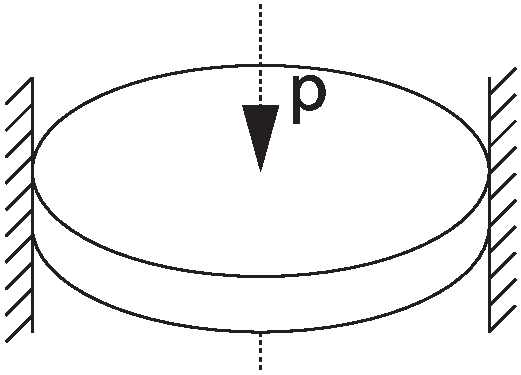
\includegraphics[width=100pt]{3D_fixed_point_NoHole.pdf}

\[y_{max} = \frac{-p R^2}{16 \pi D} \frac{3 + \nu}{1 + \nu}\]
Fixed Point No Hole
\[y_{max} = \frac{-p R^2}{16 \pi D}\]
Pinned Distributed No Hole
\[y_{max} = \frac{-q R^4 (5+ \nu)}{64D(1+\nu)}\]
Fixed Distributed No Hole
\[y_{max} = \frac{-q rR^4}{64D}\]

\section{Plate With a Hole (Washers)}
Pinned Point Hole
\[y_{max}=\frac{-p R^3}{D}\left(\frac{C_1 L_9}{C_7} - L_3\right)\]
\[C_1 = \frac{1+\nu}{2}\frac{r}{R} \ln \frac{R}{r}+\frac{1-\nu}{4} \left( \frac{R}{r} - \frac{r}{R}\right)\]
\[C_7 = \frac{1}{2} (1-\nu^2)\left( \frac{R}{r} - \frac{r}{R}\right)\]
\[L_3 = \frac{r}{4R}\left( \left(\left( \frac{r}{R} \right) ^2 +1 \right) \ln \frac{R}{r} + \left( \frac{r}{R}\right)^2 -1 \right)\]
\[L_9 = \frac{r}{R}\left( \frac{1+\nu}{2} \ln \frac{R}{r}    + \frac{1-\nu}{4}  \left( 1 - \left( \frac{r}{R} \right) ^2  \right) \right)\]
Fixed Point Hole
\[y_{max}=\frac{-p R^3}{D}\left(\frac{C_1 L_6}{C_4} - L_3\right)\]
\[C_1 = \frac{1+\nu}{2}\frac{r}{R} \ln \frac{R}{r}+\frac{1-\nu}{4} \left( \frac{R}{r} - \frac{r}{R}\right)\]
\[C_4 = \frac{1}{2} \left( (1+\nu)\frac{r}{R} + (1-\nu) \frac{R}{r} \right)\]
\[L_3 = \frac{r}{4R}\left( \left(\left( \frac{r}{R} \right) ^2 +1 \right) \ln \frac{R}{r} + \left( \frac{r}{R}\right)^2 -1 \right)\]
\[L_6 = \frac{r}{4R}\left( \left( \frac{r}{R} \right) ^2 -1+2 \ln \frac{R}{r}  \right)\]
Pinned Distributed Hole
\[y_{max}=\frac{-q R^4}{D}\left(\frac{C_1 L_{17}}{C_7} - L_{11}\right)\]
\[C_1 = \frac{1+\nu}{2}\frac{r}{R} \ln \frac{R}{r}+\frac{1-\nu}{4} \left( \frac{R}{r} - \frac{r}{R}\right)\]
\[C_7 = \frac{1}{2} (1-\nu^2)\left( \frac{R}{r} - \frac{r}{R}\right)\]
\[L_{11} = \frac{1}{64} \left(1 + 4 \left( \frac{r}{R}\right)^2 -5\left( \frac{r}{R}\right)^4 -4\left( \frac{r}{R}\right)^2\left[ 2 + \left( \frac{r}{R}\right)^2 \right] \ln  \frac{r}{R} \right) \]
\[L_{17} =\frac{1}{4} \left( 1 - \frac{1-\nu}{4} \left( 1 - \left( \frac{r}{R} \right) ^4 \right) - \left( \frac{r}{R} \right) ^2 \left( 1 + (1 + \nu ) \ln \frac{R}{r} \right) \right) \]
Fixed Distributed Hole
\[y_{max}=\frac{-q R^4}{D}\left(\frac{C_1 L_{14}}{C_4} - L_{11}\right)\]

\[C_1 = \frac{1+\nu}{2}\frac{r}{R} \ln \frac{R}{r}+\frac{1-\nu}{4} \left( \frac{R}{r} - \frac{r}{R}\right)\]
\[C_4 = \frac{1}{2} \left( (1+\nu)\frac{r}{R} + (1-\nu) \frac{R}{r} \right)\]
\[L_{11} = \frac{1}{64} \left(1 + 4 \left( \frac{r}{R}\right)^2 -5\left( \frac{r}{R}\right)^4 -4\left( \frac{r}{R}\right)^2\left[ 2 + \left( \frac{r}{R}\right)^2 \right] \ln  \frac{r}{R} \right) \]
\[L_{14} = \frac{1}{16} \left(1 - \left( \frac{r}{R}\right)^4 - 4\left( \frac{r}{R}\right)^2  \ln  \frac{R}{r}  \right)\]


\chapter{Performance Evaluation}

\chapter{Conclusions}




\end{document}